\documentclass[11pt,a4paper,oneside]{report}

% =========================================================
% Packages
% =========================================================
\usepackage[a4paper,margin=25mm]{geometry}
\usepackage[T1]{fontenc}
\usepackage[utf8]{inputenc}
\usepackage{lmodern}

\usepackage{float}
\usepackage{xcolor}
\usepackage{graphicx}
\usepackage{booktabs}
\usepackage{array}
\usepackage{longtable}
\usepackage{enumitem}
\usepackage{amsmath}
\usepackage{caption}
\usepackage{listings}
\usepackage{tcolorbox}
\usepackage{titlesec}
\usepackage{fancyhdr}
\usepackage[hidelinks]{hyperref}
\usepackage{parskip}

\newcommand{\rustlogo}{%
	\IfFileExists{images/rustlogo.png}{%
		\raisebox{-0.98em}{
\includegraphics[height=2.5em]{images/rustlogo.png}}%
	}{%
		\textbf{Rust}%
	}%
}

% =========================================================
% Colours
% =========================================================
\definecolor{ink}{HTML}{1F2937}
\definecolor{muted}{HTML}{6B7280}
\definecolor{accent}{HTML}{2563EB}
\definecolor{softaccent}{HTML}{DBEAFE}
\definecolor{codebg}{HTML}{F8FAFC}
\definecolor{rulegray}{HTML}{D1D5DB}

% =========================================================
% Page style
% =========================================================
\pagestyle{fancy}
\fancyhf{}
\lhead{\textcolor{muted}{CPS2000 Compiler Theory and Practice}}
\rhead{\textcolor{muted}{\thepage}}
\renewcommand{\headrulewidth}{0.4pt}

% =========================================================
% Chapter style
% Keeps the high chapter position and underline, but removes
% the blue square beside chapter numbers.
% =========================================================
\titleformat{\chapter}
{\normalfont\huge\bfseries\color{ink}}
{\thechapter}
{1em}
{}
[\vspace{0.4em}\titlerule]

\titlespacing*{\chapter}{0pt}{-10pt}{30pt}

% =========================================================
% General code listing style
% No language-specific syntax highlighting.
% =========================================================
\lstdefinestyle{compilerstyle}{
	backgroundcolor=\color{codebg},
	basicstyle=\ttfamily\small,
	breaklines=true,
	frame=single,
	rulecolor=\color{rulegray},
	columns=fullflexible,
	keepspaces=true,
	showstringspaces=false,
	tabsize=4,
	numbers=left,
	numberstyle=\tiny\color{muted},
}

\lstset{style=compilerstyle}

% =========================================================
% Reusable boxes
% =========================================================
\newtcolorbox{designbox}{
	colback=softaccent,
	colframe=accent,
	title= Note,
	fonttitle=\bfseries
}

\newtcolorbox{testbox}{
	colback=rulegray,
	colframe=darkgray,
	title=Testing Methodology,
	fonttitle=\bfseries
}

\newtcolorbox{riskbox}{
	colback=red!6,,
	colframe=red!60!black,
	title=Limitation / known issue,
	fonttitle=\bfseries
}

% =========================================================
% Document metadata
% =========================================================
\title{
	\vspace{-1cm}
	\Huge\textbf{ResIR Compiler Report}\\
	\vspace{0.3cm}
	\Large CPS2000 -- Compiler Theory and Practice
}
\author{
	Name: \textbf{Dave Galea}\\
	Student ID: \textbf{0283404L}\\
	Implementation Language: \rustlogo\
}
\date{June 2026}

\begin{document}
	
	% =========================================================
	% Front matter
	% =========================================================
	\maketitle
	
	\begin{abstract}
		While a report cannot fully capture all parts of this project without becoming a novel, it can provide an insight to most of the important design decisions taken throughout this assignment.
		
		This report is therefore my best attempt at expressing the work done for the fulfillment of the course CPS2000: Compiler Theory and Practice. It has discussion regarding implementation, testing, and any specifics related to a particular piece of the Compiler. Any limitations and ideas for future improvement are also included toward the end of the report. 
		
		The link for the explanation video can be found here: \url{https://drive.google.com/file/d/1rIBUSCF6zFFP6oiAW43uhfWXDCihbOWh/view?usp=sharing} 
	\end{abstract}
	
	\tableofcontents
	\newpage
	
	% =========================================================
	\chapter{Project Overview}
	
	\section{Aim}
	The goal of this project is to build a compiler pipeline for an Intermediate Representation (IR) called \texttt{ResIR}, through which \texttt{ResIR} source code is inputted, and Compilable C is outputted. 
	
	\section{Pipeline}
	The compiler pipeline structured as follows:
	
	\begin{center}
		\begin{tabular}{lll}
			\toprule
			Stage & Input & Output \\
			\midrule
			Lexical analysis & ResIR source code & Tokens \\
			Syntax analysis & Tokens & Filled Intermediate Representation + CFG \\
			Semantic analysis & Program + CFG & Result of the Check  \\
			Code generation & Program and Ascent output & C source code with no unreachable blocks \\
			Program analysis & CFG facts & Ascent output \\
			\bottomrule
		\end{tabular}
	\end{center}

	
	\section{Repository Layout}
	\begin{lstlisting}
		src/
		|-- samples.rs --> holds all test examples
		|-- test.rs --> test harness which runs the examples 
		|-- main.rs 
		|-- parser/
		|   |-- cfg.rs
		|   |-- parser_core.rs
		|   |-- ir.rs
		|   `-- mod.rs
		|-- codegen/
		|   |-- generator.rs
		|   `-- mod.rs
		|-- lexer/
		|   |-- table.rs
		|   |-- lexer_core.rs
		|   |-- tokens.rs
		|   `-- mod.rs
		|-- semantic/
		|   |-- analyser_core.rs
		|   `-- mod.rs
		`-- datalog/
			|-- datalog_analyser.rs
			`-- mod.rs
	\end{lstlisting}
	
	Credit for the above: \url{https://utilitycove.com/tools/folder-structure-generator}
	
	\section{Running and Testing the Compiler}
	\begin{designbox}
		Regarding the header file; my understanding was that it will be provided by whoever will be testing the system. The program thus optionally takes as input the name of the header file, and \textbf{adapts to the name you provide}, so if your file is called \texttt{abcdefheader.h}, and you pass it as an argument, the generated C will contain \texttt{\#include "abcdefheader.h"}
	\end{designbox}
	\begin{riskbox}
		The header argument is only optional for inputs that do not reference a custom
		type or external function. For the struct and call examples (such as examples 2
		and 3), the header \textbf{must} be passed, otherwise the generated
		\texttt{\#include} falls back to a default name and will not match the header
		the who ever is testing provides.
	\end{riskbox}
	The program takes input as follows, with the header file being optional:
	
	
	From the root directory:
		
	\begin{center}
		\texttt{cargo run -\-- <input.resir> <output.c> [header.h]}
	\end{center}
	
	This then generates a compilable C file. A self-contained function compiles and links directly with:: 
	
	\begin{center}
		\texttt{gcc -std=c11 -Wall -Wextra -pedantic filename.c}
	\end{center}
	
	A function that calls an external helper or uses a custom struct compiles as a
	translation unit, and is linked together with the file(s) defining those
	helpers and the provided header, for example:
	
	\begin{center}
		\texttt{gcc -std=c11 -Wall -Wextra -pedantic file1.c file2.c driver.c -o demo}
	\end{center}
	
	Regarding testing, a simple \texttt{cargo test} runs the entire test harness, and produces an output specifying the tests and their outcome. 
	
	
	
	
	% =========================================================
	\chapter{Lexical Analysis}
	
	
	\section{Task Overview}
	The first step in the compilation process is here: The job of this portion of the compiler is to take any ResIR source program, and transform it into tokens. 
	
	The division of labour is thus split across three files:
	
	\begin{itemize}
		\item \texttt{tokens.rs}: Definition of token data structures. 
		\item \texttt{table.rs}: DFSA states, character categories, any useful conversions (like from a state to a token), and obviously, the transition table.
		\item \texttt{lexer\_core.rs}: the scanning loop that finally produces the tokens.
	\end{itemize}
	
	This stage was by far the longest stage to implement, even though the marks allocated were smaller than other parts like the parser and the code generation. This was because a deliberate effort was made to try and make it as well prepared to add on to as possible, as I knew that as the system grew more complex, a solid base to lie on was necessary.
	
	\section{Design}
	\paragraph{A table driven approach:}\mbox{}\\
	The lexer uses a table-driven Deterministic Finite State Automaton (DFSA)[Figure~\ref{fig:lexer-dfsa}]. Having previously done a course which touched on compiler construction; the requirement for it being table was rather unintuitive, as I was more familiar with a 'direct-coded' approach using conditional logic. Regardless, a table-driven lexer helped me regarding separation of concerns of the different parts of the lexer, aswell as give me a bit of a better insight on how the DFSA ought to function. 
	
	\paragraph{Maximal Munch}\mbox{}\\
	The concept of maximal munch (or simply longest match) was implemented for outputting tokens. This was done in such a way that when several prefixes of the remaining input could form valid tokens, the lexer chooses the longest one\cite{reps1998maximalmunch}. This implementation is necessary for tokens such as \texttt{:} and \texttt{::}, where the lexer should produce a path separator when two colons appear together, rather than producing two separate colon tokens.
	
	\paragraph{Batch model}\mbox{}\\
	I got inspired by the Batch model from the incredible book Crafting Interpreters\cite{nystrom2021crafting}. Although the lecture notes follow a stream model, where the parser receives one token at a time and parses by repeatedly requesting the next token from the lexer, I opted for a batch model.  which produces an entire list of tokens in one go, after which the entire batch of tokens is parse
	
	This choice was made on the basis that in my mind, having the lexer as a seperate process which takes in a "bucket" of input and produces a "bucket" of tokens, makes more intuitive sense. This idea of "division of labour" It allowed me to reason more about how the lexer will work without having to reason about parser structure alongside it. 
	
	\begin{figure}[H]
		\centering
		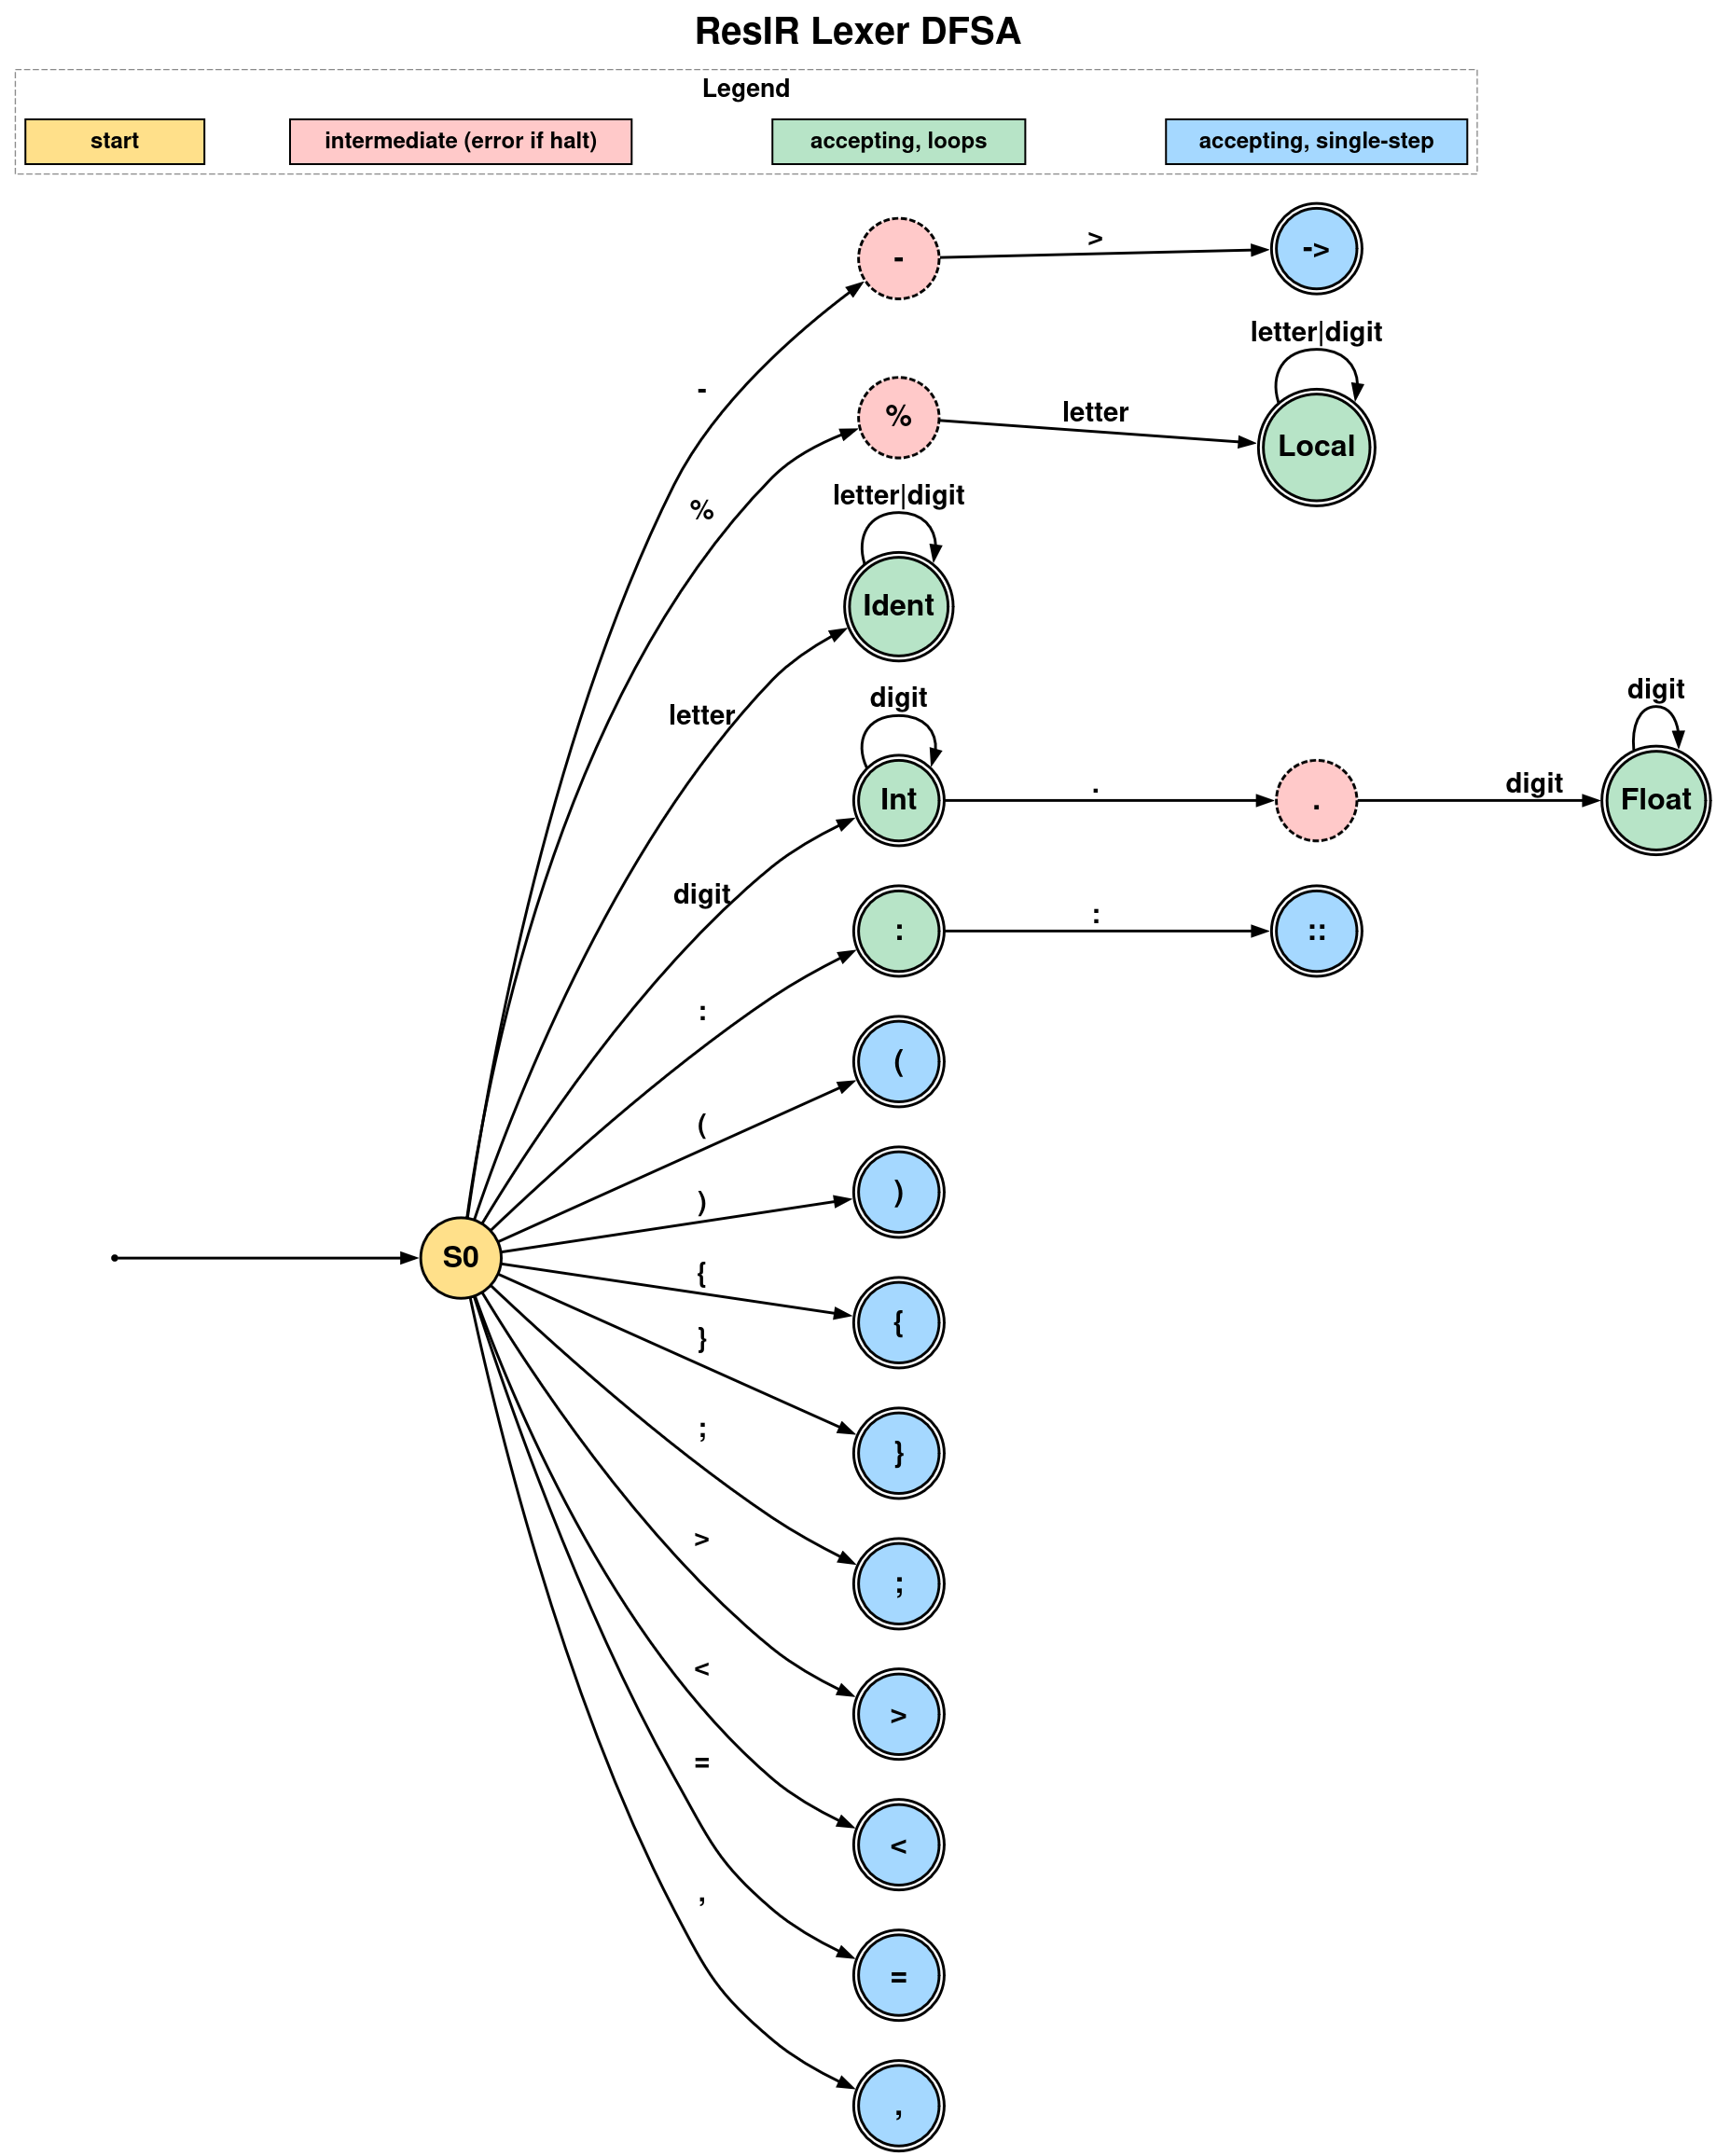
\includegraphics[width=\linewidth, height=0.8\textheight]{images/dfsa.png}
		\caption{DFSA used by the table-driven lexer}
		\label{fig:lexer-dfsa}
	\end{figure}
	\newpage
	\section{Main Functions}
	
	\begin{longtable}{p{0.30\linewidth}p{0.58\linewidth}}
		\toprule
		\textbf{Function / Structure} & \textbf{Role} \\
		\midrule
		\endhead
		
		\texttt{Token}, \texttt{TokenKind}, \texttt{TokenAttribute} &
		\texttt{TokenKind} stores the kind of token produced by the lexer, \texttt{TokenAttribute} stores the lexeme and source location, and \texttt{Token} combines both. \\
		\midrule
		
		\texttt{build\_transition\_table()} &
		Builds the DFSA transition table as follows: \texttt{table = [state][category]}.\\
		\midrule
		
		\texttt{produce\_tokens(input)} &
		This is the main lexer function, used by the rest of the compiler, which after building the transition table, loops over the input while the end of a file is not detected. In this loop, the location of the current token is tracked, \texttt{next\_token} is called repeatedly to read another lexeme. Each lexeme is checked to see whether it is a reserved keyword, or a label. If neither, it is classified as an Identifier. After the last token is read, an end of file token is appended and the full Vector of tokens is returned \\
		\midrule
		
		\texttt{next\_token(...)} &
		Scans one token: it walks the DFSA, then rolls back to the last accepting state and returns its kind and lexeme. \\
		
		\bottomrule
	\end{longtable}
	
	\section{Error Handling}
	Lexical error handling concerns finding if a character is valid or not. If the lexer finds an invalid character, it returns as follows.
	
	\begin{center}
	\texttt{Lexical Error: Unexpected character ' ' at line ' ', col ' '}
	\end{center}
	
	
	\section{Testing}
	
	\begin{testbox}
	Lexical testing revolved around confirming each token class is recognised
	correctly, and tested for keyword/label distinctions by
	asserting \texttt{(input, expected token stream)} rows through a single loop,
	with a negative test for invalid input.
	\end{testbox}
	
	\begin{longtable}{p{0.34\linewidth}p{0.54\linewidth}}
		\toprule
		\textbf{Test / Input} & \textbf{Expected outcome} \\
		\midrule
		\endhead
		Three assignment examples        & No error; stream ends in \texttt{EndOfFile} \\
		\midrule
		\texttt{\%x = const 0}          & \texttt{Local, Equals, Const, IntegerLiteral} \\
		\midrule
		\texttt{function}                & \texttt{Function}, not \texttt{Identifier} \\
		\midrule
		\texttt{bb0 bb}                  & \texttt{Label} then \texttt{Identifier} (\texttt{bb} is not a label) \\
		\midrule
		\texttt{::}       				& \texttt{::} lexes as one \texttt{PathSep}, not two \texttt{Colon}  \\
		\midrule
		\texttt{12.34}                   & single \texttt{FloatLiteral} \\
		\midrule
		\texttt{invalid characters}      & \texttt{Err} containing \texttt{"Lexical Error"} \\
		\midrule
		\texttt{function\textbackslash n~~@} & \texttt{Err} naming the correct line (2) and column (3) \\
		\bottomrule
	\end{longtable}
		
	
	% =========================================================
	\chapter{Syntax Analysis}
	
	\section{Task Overview}
	With a batch of tokens now available, the next step is to give them shape. The job of this portion of the compiler is to take the \texttt{Vec} of tokens produced by the lexer and build an in-memory representation of the program aswell as a Control Flow Graph(CFG). 
	
	The division of labour is split across three files:
	
	\begin{itemize}
		\item \texttt{ir.rs}: the IR data structures of which every node of the program is built from (\texttt{Program}, \texttt{Function}, \texttt{Block}, \texttt{Stmt}, \texttt{Rhs}, \texttt{Term}, \texttt{Type}, and so on).
		\item \texttt{parser\_core.rs}: the parser itself, with one \texttt{Parse\_x} function per grammar rule. 
		\item \texttt{cfg.rs}: builds a Control Flow Graph from the parsed program. 
	\end{itemize}
	
	\subsection{Internal Representation}
	The parser ultimately produces a \texttt{Program}. A program contains optional external type declarations and is limited to one function per program. 
	
	\begin{lstlisting}
		pub struct Program {
			pub externtypes: Vec<ExternType>,
			pub function: Function,
		}
		
		pub struct Function {
			pub path: Path,
			pub params: Option<Params>,
			pub rettype: RetType,
			pub locals: Vec<(Local, Type)>,
			pub entry: Label,
			pub blocks: Vec<Block>,
		}
	\end{lstlisting}
	

	\section{Design}
	\paragraph{A recursive descent parser:}\mbox{}\\
	
	This was another major debate on continuing with the implementation. In the previous course I followed, this time, the table-driven approach was the more familiar. We worked many examples by hand, so my familiarity drew me to it. However, as I quickly found out, knowing how to calculate something by hand does not mean it is trivial to implement it by hand, and a quick google search led me to find that table-driven parsing is one of the more difficult approaches to take. Thus, an alternative was needed. 
	
	Once again, I landed on Crafting Interpreters, which ultimately landed me on Recursive Descent. The idea is simple: For each grammar rule, the non terminal x gets parsed with a \texttt{parse\_x} function, and terminals, which follow the non-terminal, are checked to match the expected token; \textit{the expected token is based on the grammar rule the non-terminal specifies.}
	
	An example is as follows: 
	\begin{center}
		The grammar specifies \texttt{Term ::= 'jump' Label}
	\end{center}
	
		The parser proceeds to call parse\_term(), for the non terminal 'Term'(Terminator). Then, checks that the following token matches the terminal: jump. After verifying that this is correct, it calles parse\_label() for the final non terminal. 
	
	
	\paragraph{Navigation helpers}\mbox{}\\
	A small set of helper functions sits underneath the parsing rules: \texttt{peek()} to look without consuming, \texttt{advance()} to consume, \texttt{check\_tokenkind()} to test the current token, \texttt{match\_token()} to optionally consume one, and \texttt{consume\_token()} to demand a specific token, and raise an error if it doesn't match. These were once again inspired from the book Crafting Interpreters. 
	
	\paragraph{Lookahead}\mbox{}\\
	As specified in the assignment, parsing requires only one token of lookahead in \textit{almost} all cases. The one time that this is not applicable is for statements, where:
	
	\begin{center}
	\texttt{Stmt ::= [Local '='] Rhs}
	\end{center}
	
	This is handled in \texttt{parse\_stmt} by remembering the current position, peeking one token ahead to check for an \texttt{=}, and then restoring the position before actually parsing.
	\paragraph{A separate CFG}\mbox{}\\
	The parser produces a plain IR from which the Control Flow Graph is then built separately in \texttt{cfg.rs} by \texttt{build\_cfg}. Keeping CFG construction out of the parser meant the parser only had to worry about syntax, while later stages (especially Program Analysis) had a ready made graph to work over.

	\begin{lstlisting}
		pub struct Cfg {
			pub blocks: Vec<Block>,
			pub edges: Vec<(Label, Label)>,
			pub entry: Label,
		}
	\end{lstlisting}
	
	\begin{center}
		\begin{tabular}{ll}
			\toprule
			Terminator & CFG edges \\
			\midrule
			\texttt{return} & none \\
			\texttt{jump bbX} & current block $\rightarrow$ bbX \\
			\texttt{cjump \%c, bbX, bbY} & current block $\rightarrow$ \texttt{bbX}, current block $\rightarrow$ \texttt{bbY} \\
			\bottomrule
		\end{tabular}
	\end{center}
	\newpage
	
	\section{Error Handling}
	Syntax error handling concerns finding broken grammar rules, through expectation of tokens at under specific circumstances. If the Parser finds a broken grammar rule, it produces a syntax error through \texttt{yell\_error}, which returns as follows.
	
	\begin{center}
		\texttt{Syntax Error: <message> at Line: ' ', Col: ' '}
	\end{center}
	
	For example:
	
	\begin{center}
		\texttt{Syntax Error: expected ; after entry label at Line: 4, Col: 5}
	\end{center}
	
	\section{Testing}
	
	\begin{testbox}
		Syntax testing revolved around confirming that the appropriate structs in the IR are filled adequately, and that any incorrect grammar rules do not allow the compiler to continue via a syntax error.  
	\end{testbox}
	
	\begin{longtable}{p{0.34\linewidth}p{0.54\linewidth}}
		\toprule
		\textbf{Test / Input} & \textbf{Expected outcome} \\
		\midrule
		\endhead
		Three assignment examples        & Parse with no error \\
		\midrule
		\texttt{\%x = const 0}           & \texttt{Rhs::Const}; block ends in \texttt{Term::Return} \\
		\midrule
		\texttt{bin add}                 & \texttt{Rhs::Bin} \\
		\midrule
		\texttt{call Math::abs\_diff}    & \texttt{Rhs::Call} \\
		\midrule
		\texttt{member\_ptr \%p, x}      & \texttt{Rhs::Member\_ptr} \\
		\midrule
		\texttt{cjump \%c, bb1, bb2}     & \texttt{Term::CJump} \\
		\midrule
		missing \texttt{;}               & \texttt{Err} (syntax error) \\
		\midrule
		missing \texttt{entry}           & \texttt{Err} (syntax error) \\
		\bottomrule
	\end{longtable}
	
	% =========================================================
	\chapter{Semantic Analysis}
	
	\section{Task Overview}
	With a parsed program and its CFG acquired, the next step is to derive \textit{meaning} before any C is generated. It acts as a validation check that the program has to get through after parsing before being able to continue to the final stages of compilation. 
	
	Unlike the previous stages, this one lives almost entirely in a single file:
	
	\begin{itemize}
		\item \texttt{analyser\_core.rs}: a small \texttt{SymbolTable}, and a sequence of independent check functions driven by one \texttt{analyse} function.
	\end{itemize}
	
	\section{Checks Implemented}
	

	\begin{longtable}{p{0.28\linewidth}p{0.62\linewidth}}
		\toprule
		\textbf{Check} & \textbf{Description} \\
		\midrule
		Declared locals & Every local used as a destination, an operand, or in a terminator must exist in the symbol table. \\
		\midrule
		Unique labels & A block label must not appear more than once. \\
		\midrule
		Entry exists & The declared entry block must exist among the blocks. \\
		\midrule
		Targets exist & Every jump and cjump target must refer to a real block. \\
		\midrule
		Operand types & operations must use compatible types; in general a statement's left- and right-hand types must be compatible or equal. \\
		\midrule
		Return type & Every return must match the function's return type, and a void function must not return a value. \\
		\midrule
		CJump condition & A cjump condition must have type bool. \\
		\midrule
		Extern types & Every custom (path) type used by fields, parameters, the return type, locals, or a cast must have a matching extern type declaration. \\
		\bottomrule
	\end{longtable}
	
	\section{Design}
	\paragraph{A symbol table:}\mbox{}\\
	Inspired from the lecture notes, The \texttt{SymbolTable} is simply a \texttt{HashMap} from a local's name to its \texttt{Type}, filled once from the parameters and then the locals; i.e. places where declaration of variables can take place. Every later check that needs a type simply looks it up here, and a failed lookup is itself the "undeclared local" error.
	\newpage
	\begin{lstlisting}
		let mut symboltable = SymbolTable::new(); 
		if let Some(params) = &function.params {
			for param in &params.params {
				symboltable.insert(&param.local.ident.string, param.typealt.clone());
			}
		}
		for (local, typealt) in &function.locals {
			symboltable.insert(&local.ident.string, typealt.clone());
		}
	\end{lstlisting}
	
	
	\paragraph{Smaller checks over a big one}\mbox{}\\
	Rather than doing everything with one \texttt{analyse()} function which does checks at once, the work is modularly split into eight small check functions (besides the one checking for operand types which took half the file), each responsible for one kind of invariant. This kept the, in my opinion, most difficult part of the assignment a bit more manageable, and also made the testing straightforward, as it was simply a matter of testing every check. 
	
	\paragraph{Type checking statements}\mbox{}\\
	As previously mentioned, the largest stage in the semantic analyser is \texttt{check\_statements}. For the majority of statements, the rule is simply that the type of the left-hand side must equal the type of the right hand side. The left-hand side type is derived from the lookup table for the local, while for the right side the type is derived from the operation performed. 
	
	A few cases deviate from this idea, and are handled separately; notably:
	\begin{itemize}
		\item \texttt{const}, for which the type of literal is checked to be compatible with the destination, rather than equal.
		\item \texttt{store}, which has no left-hand side at all, and which is instead checked for pointer and pointee type equality
		\item \texttt{member\_ptr} for which: 
		\begin{itemize}
			\item 1) the operand must have type \texttt{ptr<P>}.
			\item 2) The path \texttt{P} must be declared by an \texttt{extern type} block.
			\item 3) The field must exist
			\item 4) The result type is \texttt{ptr<T>}, where \texttt{T} is the field type.
		\end{itemize}
	\end{itemize} 
	
	\paragraph{Using the CFG}\mbox{}\\
	Three of the checks (label uniqueness, entry block exists, and that every jump target exists) are about control-flow integrity, so they run over the \texttt{Cfg} previosuly built. Whilst this wasn't strictly necessary, it helped simplify most of the logic there was no need to rederive structure
	
	\newpage
	\section{Error Handling}
	Like the parser, the pass stops at the first problem and reports it; for example, the error for a mismatched type for CJump's condition: 
	
	\begin{center}
		\texttt{Cjump's condition type must be a boolean. Got <type> instead.}
	\end{center}
	
	\begin{riskbox}
		One limitation that will be included in the later section regarding future improvements is location handling to easily find the errors for the semantic pass. Regardless, each check returns a descriptive message naming what went wrong, as shown above. 
	\end{riskbox}
	
		
	\section{Testing}
	
	\begin{testbox}
		Semantic testing revolved around confirming that each of the proposed invariant checks worked, aswell as that a valid program such as those in the assignment spec are not wrongly rejected 
		
	\end{testbox}
	
	\begin{longtable}{p{0.40\linewidth}p{0.48\linewidth}}
		\toprule
		\textbf{Test / Input} & \textbf{Expected outcome} \\
		\midrule
		\endhead
		Three assignment examples        & \texttt{Ok}: well-formed \\
		\midrule
		Undeclared local                 & \texttt{Err}: has no type \\
		\midrule
		Duplicate block labels           & \texttt{Err}: duplicate block label \\
		\midrule
		Entry label with no block        & \texttt{Err}: entry block does not exist \\
		\midrule
		\texttt{jump} to missing label    & \texttt{Err}: targets dont exist \\
		\midrule
		\texttt{cjump} on a non-\texttt{bool} & \texttt{Err}: condition must be a boolean \\
		\midrule
		Return type mismatch             & \texttt{Err}: return type is incorrect \\
		\midrule
		\texttt{bin add} on mismatched types & \texttt{Err}: expects matching numeric operands \\
		\midrule
		\texttt{load} from a non-pointer  & \texttt{Err}: load expects a pointer \\
		\midrule
		\texttt{store} of the wrong type  & \texttt{Err}: store cannot put incorrect type \\
		\midrule
		\texttt{member\_ptr} on a missing field & \texttt{Err}: field does not exist \\
		\midrule
		Undeclared custom type           & \texttt{Err}: referenced but not declared \\
		\bottomrule
	\end{longtable}
	
	% =========================================================
	\chapter{Code Generation}
	
	\section{Task Overview}
	The Code generator is the final process in the Compilation step. It takes as input a program which has passed the validation check, and returns a string, which then, in main, is written to a file. Ultimately, this step produces a compilable C file which implements the same function as the input ResIR code. 
	
	This process, like the semantic analyser lives in a single file:
	
	\begin{itemize}
		\item \texttt{generator.rs}: builds the C source piece by piece, and contains necessary functions to convert resir to C. 
	\end{itemize}
	
	
	\section{Design}
	\paragraph{Label-based generated code}\mbox{}\\
	The generator emits label-based C using \texttt{goto} rather than trying to rebuild structured \texttt{if} or \texttt{while} statements. This was, for me, the easier choice, especially since the idea of the control flow graph, had been burned into my mind by now. The control flow follows into basic steps: each block becomes a C label, and lowering the terminators is then almost mechanical. A \texttt{jump} becomes a \texttt{goto}, a \texttt{cjump} becomes an \texttt{if/else} over two \texttt{goto}s, and a \texttt{return} stays a \texttt{return}. 
	
	\paragraph{Conditional includes}\mbox{}\\
	Instead of emitting a fixed set of headers, the generator only adds the ones the program actually uses: \texttt{<stdint.h>} when a fixed-width integer appears, \texttt{<stdbool.h>} for \texttt{bool}, \texttt{<stddef.h>} when a \texttt{null} literal is generated (for C equivalent \texttt{NULL}) Additionally, the provided custom header is included when the program references a custom type or calls an external helper.

	\paragraph{A standalone entry point}\mbox{}\\
	The assignment requires that the generated file compile with the exact command
	\texttt{gcc -std=c11 -Wall -Wextra -pedantic generated.c}. Since that
	also links an executable, a self-contained function needs a \texttt{main} to
	link on its own. The generator therefore appends a small stub \texttt{main}
	(unless the function is itself called \texttt{main}). To avoid this clashing
	with an external \texttt{main} supplied by a test driver, the stub is marked
	weak under GCC so that if another \texttt{main} is present at link
	time that takes over
	
	\paragraph{Consuming the analysis}\mbox{}\\
	The generator also takes the list of unreachable blocks found by the Datalog stage (discussed in the next chapter), and simply skips them while emitting, so dead blocks never appear.
	
	\begin{lstlisting}
	let unreachable_blocks = get_unreachables(&cfg);
	if unreachable_blocks.is_empty() {
		println!("Datalog analysis detected no unreachable blocks. Good job.\n");
	} else {
		println!("Datalog analysis eliminated {} unreachable block/s\n", unreachable_blocks.len());
	}
	let c_code = generate_c(&program, header_name, &unreachable_blocks);
	\end{lstlisting}
		
	\section{Main Functions}
	
	\begin{longtable}{p{0.30\linewidth}p{0.58\linewidth}}
		\toprule
		\textbf{Function / Structure} & \textbf{Role} \\
		\midrule
		\endhead
		
		\texttt{generate\_c(...)} &
		The main entry point. Takes as input the program, the header file name, and the uncreachable blocks generated from the following step. Assembles the full C string: includes, signature, local declarations, entry block, and each block's label, statements, and terminator.\\
		\midrule
		
		\texttt{type\_to\_c(type)} &
		For assisting with Type Mapping: it maps a ResIR type to its C equivalent. \\
		\midrule
		
		\texttt{include\_includes(...)} &
		Works out which headers the program actually needs and emits only those. \\
		\midrule
		
		\texttt{pathsepto\_(path)} &
		Joins a path's parts with underscores to form a C identifier (\texttt{A::B::C}~$\rightarrow$~\texttt{A\_B\_C}). \\
		\midrule
		
		\texttt{convert\_ops(stmt)} &
		For Operation lowering. Converts a ResIR operation to its C equivalent.\\
		\midrule
		
		\texttt{convert\_terminators(term)} &
		Lowers a terminator: \texttt{jump}~$\rightarrow$~\texttt{goto}, \texttt{cjump}~$\rightarrow$~\texttt{if/else}, \texttt{return}~$\rightarrow$~\texttt{return}. \\
		
		\bottomrule
	\end{longtable}
	\section{Type Mapping}
	\begin{center}
		\begin{tabular}{ll}
			\toprule
			ResIR type & C type \\
			\midrule
			\texttt{i32} & \texttt{int32\_t} \\
			\texttt{i64} & \texttt{int64\_t} \\
			\texttt{u32} & \texttt{uint32\_t} \\
			\texttt{f64} & \texttt{double} \\
			\texttt{bool} & \texttt{bool} \\
			\texttt{ptr<T>} & \texttt{T *} \\
			\texttt{A::B::C} & \texttt{A\_B\_C} \\
		\end{tabular}
	\end{center}
	
\section{Operation Lowering}
\begin{longtable}{p{0.30\linewidth}p{0.55\linewidth}}
	\toprule
	ResIR operation & C lowering \\
	\midrule

	\texttt{const}               & assignment to the literal (\texttt{null}~$\rightarrow$~\texttt{NULL}) \\

	\texttt{bin} (add, sub, \dots, and, or) & the matching C operator, e.g. \texttt{ +, - , \%, \&\& \dots} \\

	\texttt{un neg} / \texttt{un not} & \texttt{x = -a;} / \texttt{x = !a;} \\

	\texttt{cast \%a to T}        & \texttt{x = (T)a;} \\

	\texttt{addr\_of}            & \texttt{x = \&a;} \\

	\texttt{member\_ptr}         & \texttt{x = \&p->field;} \\

	\texttt{load}                & \texttt{x = *p;} \\

	\texttt{store}               & \texttt{*p = v;} \\

	\texttt{call}                & ordinary C call, \texttt{::}~$\rightarrow$~\texttt{\_} \\

	\texttt{jump bbX}            & \texttt{goto bbX;} \\

	\texttt{cjump \%c, bbX, bbY} & \texttt{if (c) goto bbX; else goto bbY;} \\

	\texttt{return [\%x]}        & \texttt{return x;} or \texttt{return;} \\
\end{longtable}
	
	
	\section{Testing}
	
	\begin{testbox}
		For Code Generation, there are no \textit{direct} tests from the test harness; however, some tests regarding the program analysis section which follows this require functioning program generation, therefore I decided to join the two tests to reduce unnecessary automated testing. However, that being said, this part is still tested manually, as will be shown in the video; the generated C file is tested to be compileable using the appropriate command, and the code implements the specified function correctly.  
	\end{testbox}
	
	\begin{designbox}
		The requirement for the report to include three input ResIR functions together with the generated C will be fullfilled near the end of the report, in the appendix section. 
	\end{designbox}
	% =========================================================
	% =========================================================
	
	\chapter{Program Analysis with Ascent}
	\section{Task Overview}
	The stage of program analysis involves a an analysis over the CFG built by the parser. The analysis I chose was unreachable-block detection, for similar reasons for choosing the label based lowering for code generation; familiarity with the idea of a Control Flow Graph. The analysis, after finding unreachable blocks of code(if any) then derives as set of such, which as shown beforehand, is consumable by the \texttt{generate\_c} function from code generation, so to eliminate any unreachable blocks of code
	
	
	\section{Design}
	\paragraph{Ascent}\mbox{}\\
	Given the choice of implementation with Rust, Ascent, being an embedded Datalog library \textit{for} Rust was the obvious choice. 
	
	\paragraph{Facts and rules}\mbox{}\\
	This is the clearest instance where having the CFG built from the parser task was a great time saver. The facts come straight from the CFG: Each CFG edge becomes an \texttt{edge} fact, and the entry block becomes an \texttt{entry} fact. 
	
	The Derived relation, \texttt{reachable}, is computed then by the two following rules: 
	\begin{itemize}
		\item The entry block is \textbf{always} reachable
		\item Any block reachable from a reachable block, is automatically reachable. 
	\end{itemize}
	
	\begin{lstlisting}
	// facts
	relation edge(Label, Label);
	relation entry(Label);
	
	// derived
	relation reachable(Label);
	
	// rules
	reachable(block) <-- entry(block);
	reachable(to)    <-- reachable(from), edge(from, to);
\end{lstlisting}
	
	\paragraph{Producing the Set of Unreachable Blocks}\mbox{}\\
	Ascent then runs the rules above to a fixpoint, from which it then produces the set of reachable blocks. To compute the set of \textit{un}reachable blocks, the function \texttt{get\_unreachable(cfg)} walks the full CFG's blocks, and finds any blocks not in the set of reachable blocks; any one out is defined as unreachable. 
	
	\paragraph{Output Consumable by the compiler}\mbox{}\\
	As previously mentioned during the discussion on code generation; the output of the analysis; a set of unreachable blocks, is fed into the function which generates C so to eliminate any unreachable blocks during generation. 
	
	
	\section{Testing}
	\begin{testbox}
		Testing the Program analysis involved confirming that the right blocks were confirmed to be unreachable / reachable, aswell as testing that the generated output eliminates the correct blocks. 
	\end{testbox}
	
		\begin{longtable}{p{0.44\linewidth}p{0.44\linewidth}}
		\toprule
		\textbf{Test / Input} & \textbf{Expected outcome} \\
		\midrule
		\endhead
		Block with no incoming edge        & flagged unreachable (one block) \\
		\midrule
		correct \texttt{jump} chain  & nothing unreachable \\
		\midrule
		\texttt{cjump} with both targets used & nothing unreachable \\
		\midrule
		\texttt{cjump} plus a stray block  & only the stray block unreachable \\
		\midrule
		Dead block, then generate C        & generated C omits that block's label \\
		\midrule
		Reachable blocks, then generate C  & generated C keeps \texttt{bb0}, \texttt{bb1}, \texttt{bb2} \\
		\bottomrule
	\end{longtable}
	
	
	% =========================================================
	\chapter{Concluding Notes}
	
	\section{Limitations}
		\begin{itemize}[leftmargin=*]
			\item Semantic Analysis Errors are currently not able to report location
			\item Although the tests were done with trying to cover my bases, it is realistically impossible to test for everything; this however implies that it is impossible to verify that it all works 
		\end{itemize}
	
	\section{Future Improvement}
	\begin{itemize}[leftmargin=*]
		\item Broaden test coverage as much as feasibly possible
		\item Eliminate any manual checking that happens for code generation by automating compilation of the C code
		\item Implement Structural based Code generation, potentially giving the user the option to choose between label based and structural based C
		\item Add error recovery, aswell as better more useful suggestions for the user
		\item Implementation of more than one type of program analysis, such as live-variable analysis which allows for removal of unused locals
		\item Due to this being the first project I have programmed in Rust, I am sure that the code can be \textbf{much} more performant and in areas possibly simplified
	\end{itemize}
	
	
	\section{A Note on Rust for Compiler Construction}
	
	Rust was particularly suited to this task because of its performance, pattern matching, and strong type system. Its built-in testing support also made it easy to create a test harness alongside the implementation without needing extra tools. I appreciated that Rust provided some of the structure associated with object-oriented programming, through data types and \texttt{impl} blocks, without forcing the rigid class hierarchies used in languages such as Java. Features such as \texttt{match} were useful throughout the project, especially when handling tokens, IR nodes, statements, and types. The type system and borrow checker also made the implementation more reliable, and had a very high chance that if it compiled, it functioned as expected.\cite{rustdoc}
	% =========================================================
	
	\section{Deviations from the Supplied grammar}
	
	No intentional deviations were made. The grammar was implemented as closely as possible to how it was as given.
	
	\bibliographystyle{plain}
	\bibliography{references}
	\appendix
	
	\chapter{Sample ResIR Inputs}
	
	\section{Assignment Example 1}
	\begin{lstlisting}
		function Math::abs_diff(%a: i32, %b: i32) -> i32 {
			locals {
				%zero	: i32;
				%d		: i32;
				%is_neg : bool;
				%r		: i32;
			}
			entry bb0;
			bb0:
			%zero   = const 0;
			%d  	= bin sub %a, %b;
			%is_neg = bin lt %d, %zero;
			cjump %is_neg, bb1, bb2;
			
			bb1:
			%r = un neg %d;
			return %r;
			
			bb2:
			return %d;
		}
	\end{lstlisting}
		\section{Assignment Example 2}
	\begin{lstlisting}
		extern type Custom::Struct::Point {
			x : i32;
			y : i32;
		}
		function Geom::point_x(%p: ptr<Custom::Struct::Point>) -> i32 {
			locals {
				%fp : ptr<i32>;
				%v  : i32;
			}
			entry bb0;
			
			bb0:
			%fp = member_ptr %p, x;
			%v = load %fp;
			return %v;
		}
	\end{lstlisting}
	\newpage
		\section{Assignment Example 3}
	\begin{lstlisting}
		function Client::sum_abs_diffs(%a: i32, %b: i32,
		%c: i32, %d: i32) -> i32 {
			locals {
				%dx : i32;
				%dy : i32;
				%r  : i32;
			}
			entry bb0;
			
			bb0:
			%dx = call Math::abs_diff(%a, %b);
			%dy = call Math::abs_diff(%c, %d);
			%r  = bin add %dx, %dy;
			return %r;
		}
	\end{lstlisting}
	
	\chapter{Generated C Outputs}
			\section{Assignment Example 1}
	\begin{lstlisting}
	#include <stdint.h>
	#include <stdbool.h>
	
	int32_t Math_abs_diff(int32_t a, int32_t b) {
		int32_t zero;
		int32_t d;
		bool is_neg;
		int32_t r;
		
		goto bb0;
		
		bb0:
		zero = 0;
		d = a - b;
		is_neg = d < zero;
		if (is_neg) goto bb1; else goto bb2;
		
		bb1:
		r = -d;
		return r;
		
		bb2:
		return d;
	}
	
	#if defined(__GNUC__)
	__attribute__((weak))
	#endif
	int main(void) {
		return 0;
	}

	\end{lstlisting}
			\section{Assignment Example 2}
	\begin{lstlisting}
	#include <stdint.h>
	#include "custom_header.h"
	
	int32_t Geom_point_x(Custom_Struct_Point *p) {
		int32_t *fp;
		int32_t v;
		
		goto bb0;
		
		bb0:
		fp = &p->x;
		v = *fp;
		return v;
	}
	
	#if defined(__GNUC__)
	__attribute__((weak))
	#endif
	int main(void) {
		return 0;
	}

	\end{lstlisting}
			\section{Assignment Example 3}
	\begin{lstlisting}
	#include <stdint.h>
	#include "custom_header.h"
	
	int32_t Client_sum_abs_diffs(int32_t a, int32_t b, int32_t c, int32_t d) {
		int32_t dx;
		int32_t dy;
		int32_t r;
		
		goto bb0;
		
		bb0:
		dx = Math_abs_diff(a, b);
		dy = Math_abs_diff(c, d);
		r = dx + dy;
		return r;
	}
	
	#if defined(__GNUC__)
	__attribute__((weak))
	#endif
	int main(void) {
		return 0;
	}

	\end{lstlisting}
	
	
	\chapter{Full Test Harness Output}
	
	\begin{lstlisting}
	running 28 tests
	test test::binary_operation_parses ... ok
	test test::cjump_parses ... ok
	test test::const_assignment_parses ... ok
	test test::function_call_parses ... ok
	test test::lexer_returns_error_for_bad_characters ... ok
	test test::member_ptr_parses ... ok
	test test::lexer_produces_correct_tokens ... ok
	test test::missing_entry_doesnt_parse ... ok
	test test::no_semicolon_doesnt_parse ... ok
	test test::semantic_rejects_bad_bin_operands ... ok
	test test::semantic_rejects_cjump_non_bool ... ok
	test test::semantic_rejects_duplicate_labels ... ok
	test test::semantic_rejects_load_from_non_pointer ... ok
	test test::parser_passes_assignment_examples ... ok
	test test::semantic_rejects_member_ptr_missing_field ... ok
	test test::semantic_rejects_missing_entry_block ... ok
	test test::semantic_passes_assignment_examples ... ok
	test test::semantic_rejects_missing_jump_target ... ok
	test test::semantic_rejects_store_wrong_value_type ... ok
	test test::semantic_rejects_undeclared_custom_type ... ok
	test test::semantic_rejects_return_type_mismatch ... ok
	test test::task5_branch_all_reachable ... ok
	test test::task5_keeps_reachable_blocks_in_generated_c ... ok
	test test::semantic_rejects_undeclared_local ... ok
	test test::task5_branch_with_dead_block ... ok
	test test::task5_removed_block_is_not_in_generated_c ... ok
	test test::task5_returns_empty_when_all_blocks_reachable ... ok
	test test::task5_detects_unreachable_block ... ok
	
	test result: ok. 28 passed; 0 failed; 0 ignored; 0 measured; 0 filtered out; finished in 0.00s

	\end{lstlisting}
	
		\chapter{output\_checker.c used in video}
	
	\begin{lstlisting}
	#include <stdio.h>
	#include <stdint.h>
	#include "custom_header.h"
	
	int main(void) {
		int32_t r1a = Math_abs_diff(7, 3);
		int32_t r1b = Math_abs_diff(3, 7);
		
		int32_t r2 = Client_sum_abs_diffs(7, 3, 2, 9);
		
		Custom_Struct_Point p;
		p.x = 5;
		p.y = 8;
		int32_t r3 = Geom_point_x(&p);
		
		printf("Example 1a: Math_abs_diff(7, 3)\n");
		printf("Expected: 4\n");
		printf("Got:      %d\n\n", r1a);
		
		printf("Example 1b: Math_abs_diff(3, 7)\n");
		printf("Expected: 4\n");
		printf("Got:      %d\n\n", r1b);
		
		printf("Example 2: Client_sum_abs_diffs(7, 3, 2, 9)\n");
		printf("Expected: 11\n");
		printf("Got:      %d\n\n", r2);
		
		printf("Example 3: Geom_point_x({x = 5, y = 8})\n");
		printf("Expected: 5\n");
		printf("Got:      %d\n", r3);
		
		return 0;
	}
		
	\end{lstlisting}
	
\end{document}
